\chapter{Results and Discussion}
\label{chap:evaluation}

Description of chapter...



\section{Machine Learning Results}

This section discusses the results of the machine learning experiments with common machine learning models using computed feature values as input. As evaluation-method 10-fold cross validation has been chosen. Figure ... shows the comparison of several machine learning models with different parameters in terms of accuracy, precision and recall of the "parking car"-class and the necessary runtime to learn the model.




Comparison of all tested algorithms -> accuracy -> different feature sets -> Graphics

Description of Graphic

Maybe binary classification

Filtered Dataset -> Parking Space Maps

Stacked Classifier


\section{Deep Learning Results}

Same as Machine Learning REsults





\section{Comparison to existing Parking Detection Systems}

The existing prototype of a parking detection system which is closest related to the prototype presented in this thesis is the ParkNet prototype developed by Mathur et al \cite{Mathur:2010:PDS:1814433.1814448}. ParkNet uses a similar system to detect parking cars. It measures the distance to the right side to the road using an ultrasonic distance sensor and tries to find dips in the sensor signal, which represent parking cars. However, ParkNet was only developed and designed for a very restrictive area of road side streets. The evaluation data only consisted of measurements on single-lane streets with parallel parking cars. 

The main goal of this thesis is to develop a drive-by parking detection system, which can handle various different situations in city traffic, like for example driving on multi-lane streets, overtaking other vehicles, traffic jams and waiting at traffic lights. While gathering the dataset, all of these situations were faced and our prototype is trained to detect them.

ParkNet uses only two features to detect parking spaces in their approach, namely the length of segments and the distance from the sensing vehicle. Mathur et al. derived thresholds for both features with a minimum error to classify the segments in parking cars and other objects. This technique is sufficient for their simple scenario because of their restricted test data. However, on a more complicated dataset which is used in this thesis the results will probably be much worse.


\begin{figure}
	\centering
	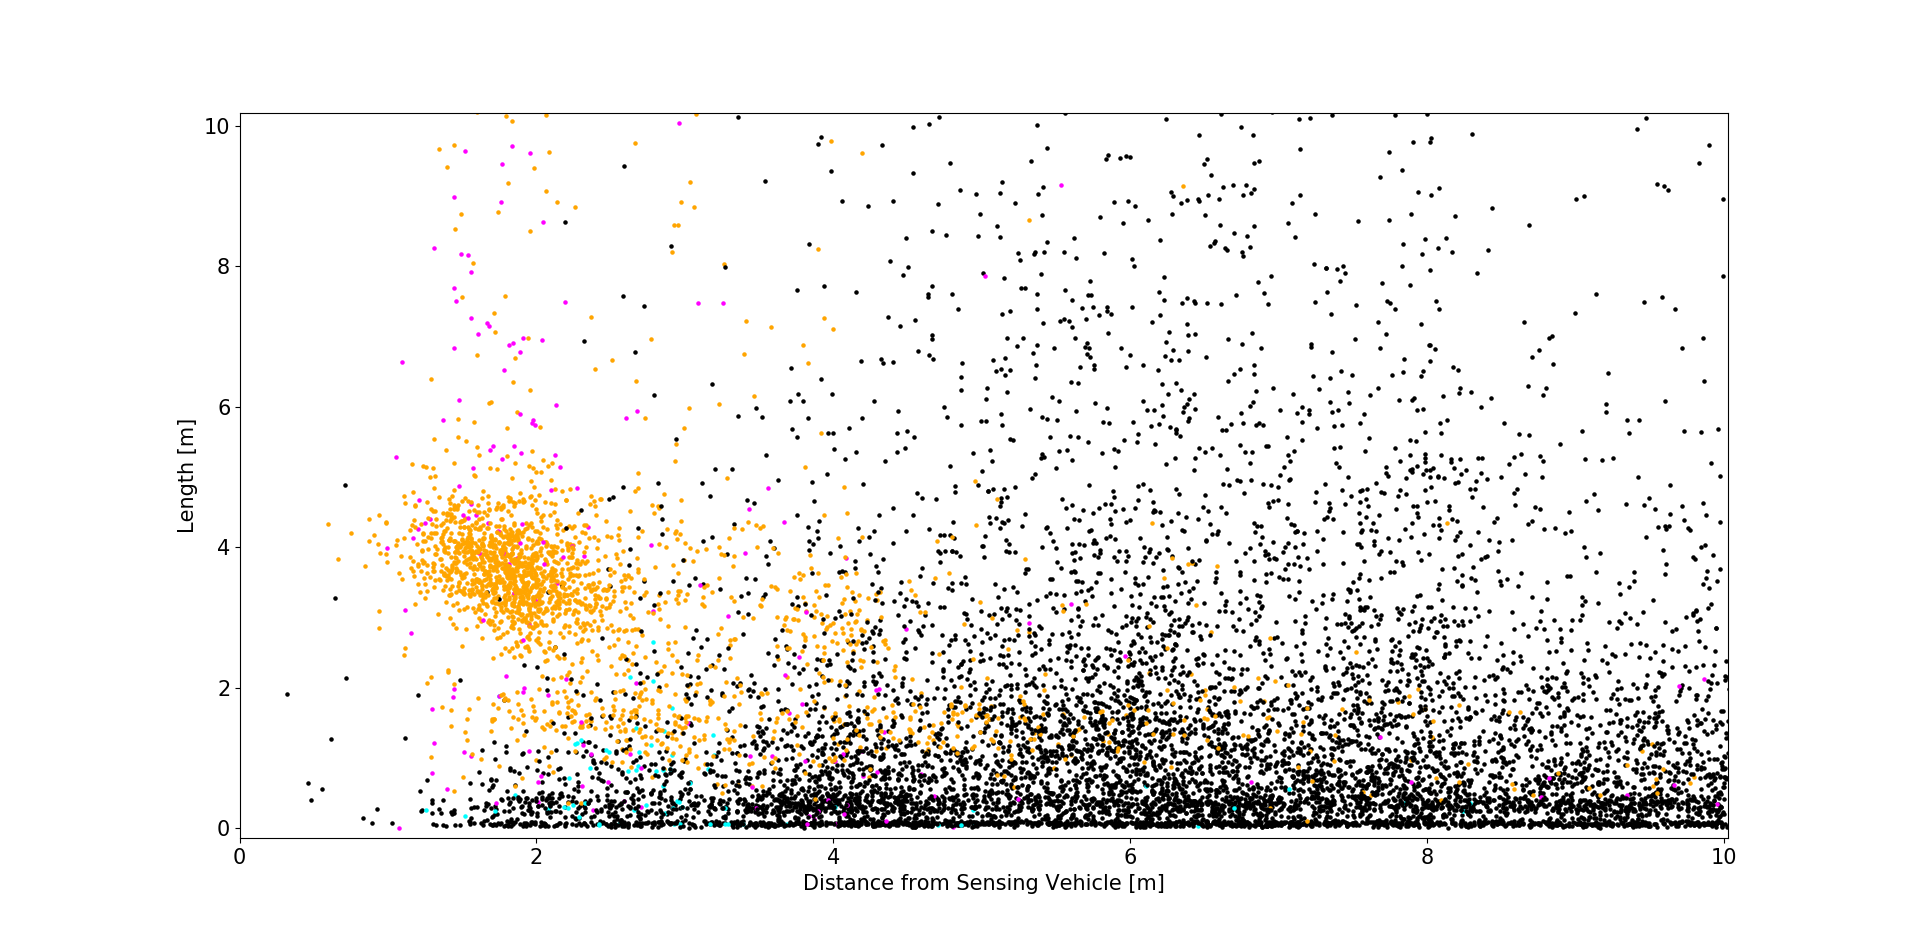
\includegraphics[width=\textwidth]{img/2d_length_distance_scatter_full_dataset.png}
	\caption{A plot of the length and distance of the segments of the full dataset. Orange points show parking cars, while black points show free spaces.}
	\label{fig:densely_dl_network}
\end{figure}

Using only the two features used in ParkNet - Which accuracy can be reached on our dataset.

ca 75\% recall and precision using ParkNet-approach